% !TeX document-id = {2870843d-1baa-4f6a-bd0a-a5c796104a32}
% !BIB TS-program = biber
% !TeX encoding = UTF-8
% TU Delft beamer template

\documentclass[aspectratio=169]{beamer}
\usepackage[english]{babel}
\usepackage{csquotes}
\usepackage{calc}
\usepackage[absolute,overlay]{textpos}
\usepackage{graphicx, subfig}
\usepackage{mathtools, amsfonts, amsthm}
\usepackage{comment}
\usepackage{siunitx}
\usepackage{MnSymbol,wasysym}
\usepackage{array}
\usepackage{qrcode}
\usepackage{hyperref}
\usepackage{setspace}
\setstretch{1.5}

\setbeamertemplate{navigation symbols}{} % remove navigation symbols
\mode<presentation>{\usetheme[verticalbar=false]{tud}}

% BIB SETTINGS
\usepackage[
    backend=biber,
    giveninits=true,
    maxnames=30,
    maxcitenames=20,
    uniquename=init,
    url=false,
    style=authoryear,
    dashed=false
]{biblatex}
\addbibresource{bib.bib}
\setlength\bibitemsep{0.3cm} % space between entries in the reference list
\renewcommand{\bibfont}{\normalfont\scriptsize}
\setbeamerfont{footnote}{size=\tiny}
%\renewcommand{\cite}[1]{\footnote<.->[frame]{\fullcite{#1}}}
\setlength{\TPHorizModule}{\paperwidth}
\setlength{\TPVertModule}{\paperheight}

\newcommand{\absimage}[4][0.5,0.5]{%
	\begin{textblock}{#3}%width
		[#1]% alignment anchor within image (centered by default)
		(#2)% position on the page (origin is top left)
		\includegraphics[width=#3\paperwidth]{#4}%
\end{textblock}}

\newcommand{\mininomen}[2][1]{{\let\thefootnote\relax%
	\footnotetext{\begin{tabular}{*{#1}{@{\!}>{\centering\arraybackslash}p{1em}@{\;}p{\textwidth/#1-2em}}}%
	#2\end{tabular}}}}

\title[]{Computational Science M.S. Thesis Proposal \\ \quad \vspace{-0.25in}\\ \emph{Production of massless spin-0 particles in analog (3+1)-dimensional de Sitter universes from a ground state BEC using high-performance computing}}
\institute[]{Central Washington University}
\author{Nathaniel W. Chapman}
%\date{}

\begin{document}
    \section*{Front Matter}
        {
        \setbeamertemplate{footline}{\usebeamertemplate*{minimal footline}}
        \frame{\titlepage}
        }

        % \begin{frame}{Contents}
        %     \tableofcontents
        % \end{frame}
        
\section{Introduction}

    \subsection{The story so far}
    
        \begin{frame}{The story so far - Analog Universes}
            \begin{enumerate}
                \item Big Bang and rapid expansion $\implies$ could observe particles
                \item Big Bang was 14 billion years ago $\implies$ we can't observe particles
                \item Condensed matter dynamics match particle dynamics (see Methods)
                \item Can make condensed matter in the lab $\implies$ can effectively observe Big Bang particles
                \item Lab based condensed matter system = ``analog universe''
            \end{enumerate}
        \end{frame}

        \begin{frame}{The story so far - Previous Research}
            Previous research has been done investigating a variety of different systems
            \begin{enumerate}
                \item ``Hyper-phononic'' quasiparticles and Lorentz Violation%\cite{Nonlinear_dispersion_Lorentz_breaking_1, Nonlinear_dispersion_Lorentz_breaking_2, Nonlinear_dispersion_Lorentz_breaking_3}
                \item Analog massive particles%\cite{massive_1, massive_2, massive_3}
                \item Analog particles with non-zero quantum spin%\cite{massive_and_spin_4, massive_and_spin_5, massive_and_spin_6, massive_and_spin_7}
                \item Analog universes with different expansion behavior%\cite{sudden_transition_1, sudden_transition_2, cyclic_cosmology, Experimental_interaction_strength_1}
                \item Analog universes with non-zero background velocity%\cite{background_velocity_1, background_velocity_2, background_velocity_3, background_velocity_4, background_velocity_5}
                \item Experimental realizations (some extremely relevant and recent)%\cite{Experimental_candidate_1, Experimental_candidate_2, Experimental_interaction_strength_1, Experimental_interaction_strength_2}
            \end{enumerate}
        \end{frame}

        \begin{frame}{The story so far - 2D \& Low-Performance Computing}
            \begin{enumerate}
                \item Analog (2+1)-dimensional universe with massless, scalar particles in a de Sitter expansion has been investigated
                \item Previous investigation provides theory and guide for conceptual analysis
                \item 3d analog universe needs high-performance computing because of increased size of wave vector domain (see Methods)
                \item Without 3d, 2d error is unknown
            \end{enumerate}
        \end{frame}
        
    \subsection{My Story}
    
        \begin{frame}{My story}
            My focus is on
            \begin{enumerate}
                \item (3+1)D analog universe with high-performance computing
                \item linear dispersion \& phononic quasiparticle
                \item analog massless particles
                \item analog spin-0 particles
                \item analog de Sitter expansion
                \item no background velocity
            \end{enumerate}
        \end{frame}

\section{Goals}

    \begin{frame}{Goals}
        \begin{enumerate}
            \item Provide insight into the dynamics of particles created due to the expansion of the universe in the moments just after the Big Bang.
            \item Quantitatively describe the error in using a reduced-dimensional physical model as compared to a full-dimensional model.
            \item Quantitatively describe the efficiency of using a full-dimensional model with high-performance computing.
            \item Provide an open-access, ``ready to use'', packaged, high-performance computational model.
        \end{enumerate}
    \end{frame}

\section{Methods}

    \begin{frame}{Methods Overview}
        \begin{enumerate}
            \item Physical Theory
                \begin{enumerate}
                    \item Setting up the Analog
                    \item Speed of Sound \& Universe Expansion
                    \item The Field Equation in Context
                    \item Particle Production
                    \item Computational Parameters
                \end{enumerate}
            \item Computation
                \begin{enumerate}
                    \item Computational Algorithms
                    \item Programming Language
                \end{enumerate}
        \end{enumerate}
    \end{frame}

    \subsection{Physical Theory}

        \subsubsection{Setting up the Analog}

            \begin{frame}{Methods - Physical Theory - Setting up the analog}
                \begin{enumerate}
                    \item Tangible: Ground state Bose-Einstein condensate with no thermal or quantum fluctuations
                    \item Mathematical: Gross-Pitaevskii equation (GPE) under a Bogoliubov mean-field approximation (aka the \textit{nonlinear Schr{\"o}dinger equation}),
                        
                        \begin{equation} \label{eq:GPE}
                            i \hbar \partial_t \psi(\mathbf{x}, t) = \left[ -\frac{\hbar^2}{2 m} \nabla^2 + V_\text{ext}(x) + U \left| \psi(\mathbf{x}, t) \right|^2 \right] \psi(\mathbf{x}, t).
                        \end{equation}
                \end{enumerate}
            \end{frame}
        
            \begin{frame}{Methods - Physical Theory - Setting up the analog}
                \begin{enumerate}
                    \item Substitute the linearized Madelung density-phase representation (below) into eq. (\ref{eq:GPE})
            
                        \begin{equation} \label{eq:Madelung}
                            \psi(\mathbf{x}, t) = \sqrt{n_0 + \hat{n}(\mathbf{x}, t)} e^{i \left( \theta_0 + \hat{\theta}(\mathbf{x}, t) \right)}
                        \end{equation}
                        
                    \item Yields the phase field equation in $d$ spatial dimensions ($g \coloneqq \text{det} \, g_{\mu \nu}$)
                    %\vspace{-0.2in}
                        \begin{exampleblock}{\centering The Field Equation}
                        \begin{equation} \label{eq:KG}
                            \frac{1}{\sqrt{-g}} \partial_\mu \left[ \sqrt{-g} g^{\mu \nu} \partial_\nu \hat{\theta} \right] = 0
                            \qquad
                            g_{\mu \nu} = \left( \frac{n_0}{c(t)} \right)^{2 / (d - 1)} \begin{bmatrix}
                                -c(t)^2 & \vdots & 0 \\
                                \cdots & & \cdots \\
                                0 & \vdots & \delta_{ij}
                            \end{bmatrix}
                        \end{equation}
                        \end{exampleblock}
                \end{enumerate}
            \end{frame}
        
            \begin{frame}{Methods - Physical Theory - Setting up the analog}
            \begin{alertblock}{\centering The Analog}
                The field equation describes the dynamics of
                \begin{itemize}
                    \item the phase of collective oscillations in the BEC
                    \item particles produced due to the expansion of the universe
                \end{itemize}
            \end{alertblock}
            \begin{exampleblock}{\centering The Field Equation}
                        \begin{equation*}
                            \frac{1}{\sqrt{-g}} \partial_\mu \left[ \sqrt{-g} g^{\mu \nu} \partial_\nu \hat{\theta} \right] = 0
                            \qquad
                            g_{\mu \nu} = \left( \frac{n_0}{c(t)} \right)^{2 / (d - 1)} \begin{bmatrix}
                                -c(t)^2 & \vdots & 0 \\
                                \cdots & & \cdots \\
                                0 & \vdots & \delta_{ij}
                            \end{bmatrix}
                        \end{equation*}
                        \end{exampleblock}
            \end{frame}

        \subsubsection{Speed of Sound \& Universe Expansion}

            \begin{frame}{Methods - Physical Theory - Speed of Sound \& Universe Expansion}
            
                \begin{alertblock}{\centering Speed Analog}
                    $\text{Speed of sound in BEC} = c(t) = \text{Speed of light in analog universe}$
                \end{alertblock}
                    
                \begin{enumerate}
                    \item Define $c(t)$ in the context of BEC
                        \begin{equation} \label{eq:speed}
                            c(t)^2 = \frac{U(t) n_0}{m} = \frac{4 \pi \hbar^2}{m^2} n_0 a(t)
                        \end{equation}
                        
                    \item  Scaling function $b(t)$
                        \begin{equation}
                            \overbrace{U(t) = U_0 b(t)}^\text{BEC Interaction Strength} \implies \overbrace{c(t) = c_0 \sqrt{b(t)}}^\text{Analog Universe Light Speed}
                        \end{equation}
                \end{enumerate}
            \end{frame}
        
            \begin{frame}{Methods - Physical Theory - Speed of Sound \& Universe Expansion}
                \begin{itemize}
                    \item A decreasing speed of light is indistinguishable from an expanding universe (i.e. $c^\prime(t) \propto 1 / \text{expansion}$)
                    
                    \begin{alertblock}{\centering Expansion Analog}
                        A decreasing BEC interaction strength yields an expanding analog universe
                    \end{alertblock}
                        
                    \item Can tune interaction strength in the lab to induce a specific expansion
        
                    \item $b(t)$ defines the expansion
                \end{itemize}
            \end{frame}

        \subsubsection{The Field Equation in Context}

            \begin{frame}{Methods - Physical Theory - The Field Equation in Context}
                \begin{enumerate}
                    \item Explicitly expansion dependent phase field equation in (2+1)D (left) and conformal time (right)
                        \begin{equation} \label{eq:fieldEquation}
                            \partial_\eta^2 \hat{\theta} - \frac{1}{2} \frac{b^\prime(\eta)}{b(\eta)} \partial_\eta \hat{\theta} - c_0^2 \nabla^2 \hat{\theta} = 0
                            \qquad 
                            d\eta = \sqrt{b(t)} dt
                        \end{equation}
                    \item Field Fourier Expansions in wave vector $\mathbf{k}$
                        \begin{subequations} \label{eq:FourierExpansion}
                        \begin{equation}
                            \hat{\theta}(\mathbf{x}, t) = \frac{1}{\sqrt{V}} \sum_\mathbf{k} e^{i \mathbf{k} \cdot \mathbf{x}} \chi_\mathbf{k}(t) \hat{b}_\mathbf{k}(t) + e^{-i \mathbf{k} \cdot \mathbf{x}} \chi_\mathbf{k}^*(t) \hat{b}_\mathbf{k}^\dagger(t)
                        \end{equation}
                        \begin{equation}
                            \hat{n}(\mathbf{x}, t) = \frac{1}{\sqrt{V}} \sum_\mathbf{k} e^{i \mathbf{k} \cdot \mathbf{x}} n_\mathbf{k}(t) \hat{b}_\mathbf{k}(t) + e^{-i \mathbf{k} \cdot \mathbf{x}} n_\mathbf{k}^*(t) \hat{b}_\mathbf{k}^\dagger(t)
                        \end{equation}
                        \end{subequations}
                \end{enumerate}
            \end{frame}

            \begin{frame}{Methods - Physical Theory - The Field Equation in Context}
                \begin{enumerate}\addtocounter{enumi}{2}
                    \item Choose de Sitter expansion for early universe ($t_s$ is the ``rate of expansion'')
                        \begin{equation}
                            b(t) = e^{-t/t_s}, \qquad 0 \leq t \leq t_f
                        \end{equation}
                        \vspace{-0.5in}
                    \item Phase Field equation with de Sitter expansion
                        \begin{exampleblock}{\centering The Fourier de Sitter Field Equation}
                            \begin{equation} \label{eq:fieldEquationdeSitter}
                                \partial_\eta^2 \chi_\mathbf{k} - \frac{1}{\eta} \partial_\eta \chi_\mathbf{k} + c_0^2 k^2 \chi_\mathbf{k} = 0
                            \end{equation}
                        \end{exampleblock}
                    \item Initial conditions from the continuity of $\chi_\mathbf{k}$ and $n_\mathbf{k} = - \frac{\hbar}{U} \partial_t \chi_\mathbf{k}$ at $t = 0$.
                \end{enumerate}
            \end{frame}

        \subsubsection{Particle Production}

            \begin{frame}{Methods - Physical Theory - Particle Production}
                \begin{enumerate}
                    \item Can represent phase and density amplitudes in same basis
                        \begin{subequations} \label{eq:mixedFourierAmplitudes}
                        \begin{equation}
                            u_k(t) = \frac{1}{2 \sqrt{n_0}} n_k(t) + i \sqrt{n_0} \chi_k(t)
                        \end{equation}
                        \begin{equation}
                            v_k(t) = \frac{1}{2 \sqrt{n_0}} n_k(t) - i \sqrt{n_0} \chi_k(t),
                        \end{equation}
                        \end{subequations}
                    \item Find $u_k(t)$ and $v_k(t)$ out of and during the expansion
                        \begin{exampleblock}{\centering Particle Production}
                            \begin{equation} \label{eq:particleProduction}
                                N_k(t) = \left| u_k^{\text{out} *}(t) v_k^{\text{exp} *}(t) - v_k^{\text{out} *} u_k^{\text{exp} *}(t) \right|^2
                            \end{equation}
                        \end{exampleblock}
                \end{enumerate}
            \end{frame}

            \begin{frame}{Methods - Physical Theory - Particle Production Algorithm}
                \begin{enumerate}
                    \item Solve the Fourier de Sitter field equation (\ref{eq:fieldEquationdeSitter}) for $\chi_\mathbf{k}(t)$ at a point in space $\mathbf{x}$
                    \item Differentiate $\chi_\mathbf{k}(t)$ to get $n_\mathbf{k}(t)$
                    \item Combine $\chi_\mathbf{k}(t)$ and $n_\mathbf{k}(t)$ to get the mixed Fourier amplitudes as in equations (\ref{eq:mixedFourierAmplitudes})
                    \item Calculate the number of particles at position $\mathbf{x}$ at time $t$ with wave vector $\mathbf{k}$ as in equation (\ref{eq:particleProduction})
                \end{enumerate}
            \end{frame}

            \begin{frame}{Methods - Physical Theory - Computational Parameters}
                %\vspace{-0.2in}
                \begin{table}[h]
                    \centering
                    \begin{tabular}{c|c|c}
                        & Previous & New  \\
                        \hline
                        Universe Size $\mathbf{x}$      & $128 \times 128$ & $128 \times 128 \times 128$ \\
                        \hline
                        Time Scale $t_s$                & $10^{-5}$ to $10^{-3}$ & $10^{-5}$ to $10^{-3}$ \\
                        \hline
                        Wave Vector Domain $\mathbf{k}$ & $||\mathbf{k}|| \leq 32 \times 2 \pi$ & $||\mathbf{k}|| < k_c$ \\
                    \end{tabular}
                    \caption{Previous and new computational domains}
                    \label{tab:Domains}
                \end{table}
                \vspace{-0.2in}
                \begin{itemize}
                    \item This system only valid for $||\mathbf{k}|| < k_c$ such that $\hbar^2 k_c^2 / 2 m = U n_0$
                    \item Time step such that the total particle number for the entire field changed by much less than one, or that the change in norm was small enough i.e. $\Delta t : \Delta ||\psi(\mathbf{x}, t)|| \leq 10^{-9}$
                \end{itemize}
            \end{frame}

    \subsection{Computational Methods}

        \begin{frame}{Methods - Computational Methods - Algorithms \& Hardware}
            \begin{table}[h]
                \centering
                \begin{tabular}{c|c}
                    \textbf{Physics} & \textbf{Method} \\
                    \hline
                    Fourier Field Equation & 4-th order Runga-Kutta \\
                    \hline
                    Density-Phase Transformation & 4-th order explicit central FD \\
                    \hline
                    Particle Production & vectorized arithmetic
                \end{tabular}
                \caption{Computational methods}
                \label{tab:methods}
            \end{table}
            \vspace{-0.2in}
            Use the ``Turing'' supercomputer for its
            \begin{itemize}
                \item ``tight''-cluster configuration
                \item dedicated head, storage, and several compute nodes
                \item NVIDIA GPUs allowing for CUDA massive parallel computing
            \end{itemize}
        \end{frame}

        \begin{frame}{Methods - Computational Methods - Programming Language}
            \vspace{-0.15in}
            \begin{itemize}
                \item Will choose between Mathematica or Julia programming languages considering the following:
                \begin{table}[c|c|c|c|c|c|c|c]
                    \centering
                    \hspace{-0.5in}
                    \begin{tabular}{c|c|c|c|c|c|c|c}
                                    & Experience & Open-source & Free & Scientific & Parallel & Cluster & GPU \\
                        \hline
                        Mathematica & X          &             &      & X          & X        & X       & X \\
                        \hline
                        Julia       &            & X           & X    & X          & X        & ?       & X
                    \end{tabular}
                    \caption{Language comparison}
                \end{table}
                \vspace{-0.25in}
                \item Other high-performance languages like C++ and Java could also be considered if performance is needed
                \item Mathematica is not good for reproducibility
            \end{itemize}
        \end{frame}

\section{Timeline}

    \begin{frame}{Timeline Overview}
        \begin{enumerate}
            \item Performance Scaling Phase - Summer '23 
            \item Domain Scaling Phase - Fall '23
            \item Writing Phase - Winter '24 
            \item Dissemination Phase - Spring '24
        \end{enumerate}
    \end{frame}

    \begin{frame}{Timeline - Performance Scaling Phase - Summer '23}
        \begin{enumerate}
            \item Convert hybrid analytic-numerical algorithms to fully numeric low-performance algorithms (LPNA) in final language of choice
            \item Test the LPNAs in the 2D model and compare against previous results%\cite{Jain}
            \item Translating the LPNAs to high-performance fully-numerical algorithms (HPNA) that make use of high-performance hardware
            \item Test the HPNAs in the 2D model and compare against previous results, measuring the efficiency when compared to the LPNA
        \end{enumerate}
    \end{frame}

    \begin{frame}{Timeline - Domain Scaling Phase - Fall '23}
        \begin{enumerate}
            \item Convert 2D theory to 3D
            \item If not generalized, convert the 2D HPNAs to 3D
            \item Test the 3D HPNAs on a small spatial domain and small momentum domain
            \item Test the 3D HPNAs on a small spatial domain and large momentum domain
            \item Do the ``real'' run of the 3D HPNAs on a large spatial domain and large momentum domain
            \item Revise and repeat runs until satisfactory results are achieved.
        \end{enumerate}
    \end{frame}

    \begin{frame}{Timeline - Writing \& Dissemination Phases - Winter \& Spring '24}
        \begin{enumerate}
            \item Writing Phase - Winter '24
                \begin{enumerate}
                    \item Write report
                    \item Prepare for conferences
                \end{enumerate}
            \item Dissemination Phase - Spring '24
                \begin{enumerate}
                    \item Defend thesis
                    \item Present at conferences
                    \item Submit final document to be considered for journal publication and graduation
                \end{enumerate}
        \end{enumerate}
    \end{frame}

\section{Anticipated Results}

    \begin{frame}{Anticipated Results}
        Refer back to goals
        \begin{itemize}
            \item Insight into particle production during the moments just after the Big Bang
            \item Quantitatively describe the error in lower-dimensional models
            \item Quantitatively describe the worth of using full-dimensional model with high-performance computing
        \end{itemize}
    \end{frame}

    \begin{frame}{Anticipated Results - Particle Production Insight}
        \begin{itemize}
            \item 2D and 3D field equations are qualitatively equal
                \begin{subequations}
                \begin{equation}
                    \hspace{-0.5in}\text{2D: } \partial_t^2\theta - \frac{3}{2} \frac{b^\prime(t)}{b(t)} \partial_t \theta - c_0^2 b(t) \nabla^2\theta = 0
                \end{equation}
                \begin{equation}
                    \hspace{-0.5in}\text{3D: } \partial_t^2\theta - \phantom{\frac{3}{2}} \frac{b^\prime(t)}{b(t)} \partial_t \theta - c_0^2 b(t) \nabla^2\theta = 0
                \end{equation}
                \end{subequations}
            \item I expect qualitatively similar results from previous research
        \end{itemize}
    \end{frame}

    \begin{frame}{Anticipated Results - Low-dimensional Model Error}
        \begin{itemize}
            \item Qualitatively similar results should yield small error
            \item Will determine how small
            \item Small enough to not warrant future research using HPC based 3D model?
            \item Big enough that more accurate results are sometimes warranted?
        \end{itemize}
    \end{frame}

    \begin{frame}{Anticipated Results - Efficiency}
        \begin{itemize}
            \item Recreated analytic 2D results
                \begin{figure}[h]
                    \centering
                    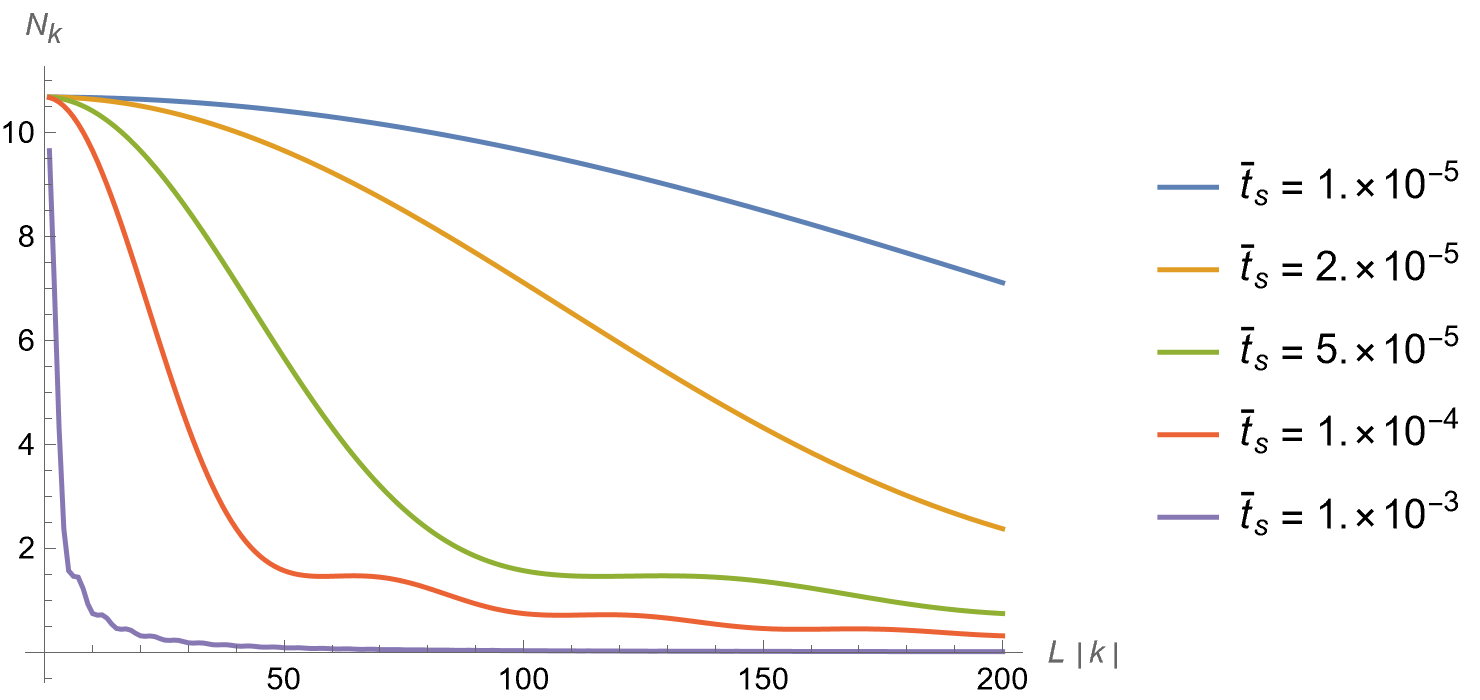
\includegraphics[width=0.75\textwidth]{fig2.png}
                    \caption{The momentum distribution when the universe stops expanding for multiple effective rates of expansion}
                    \label{fig:finalTime}
                \end{figure}
        \end{itemize}
    \end{frame}

    \begin{frame}{Anticipated Results - Efficiency}
        \begin{figure}[h]
            \centering
            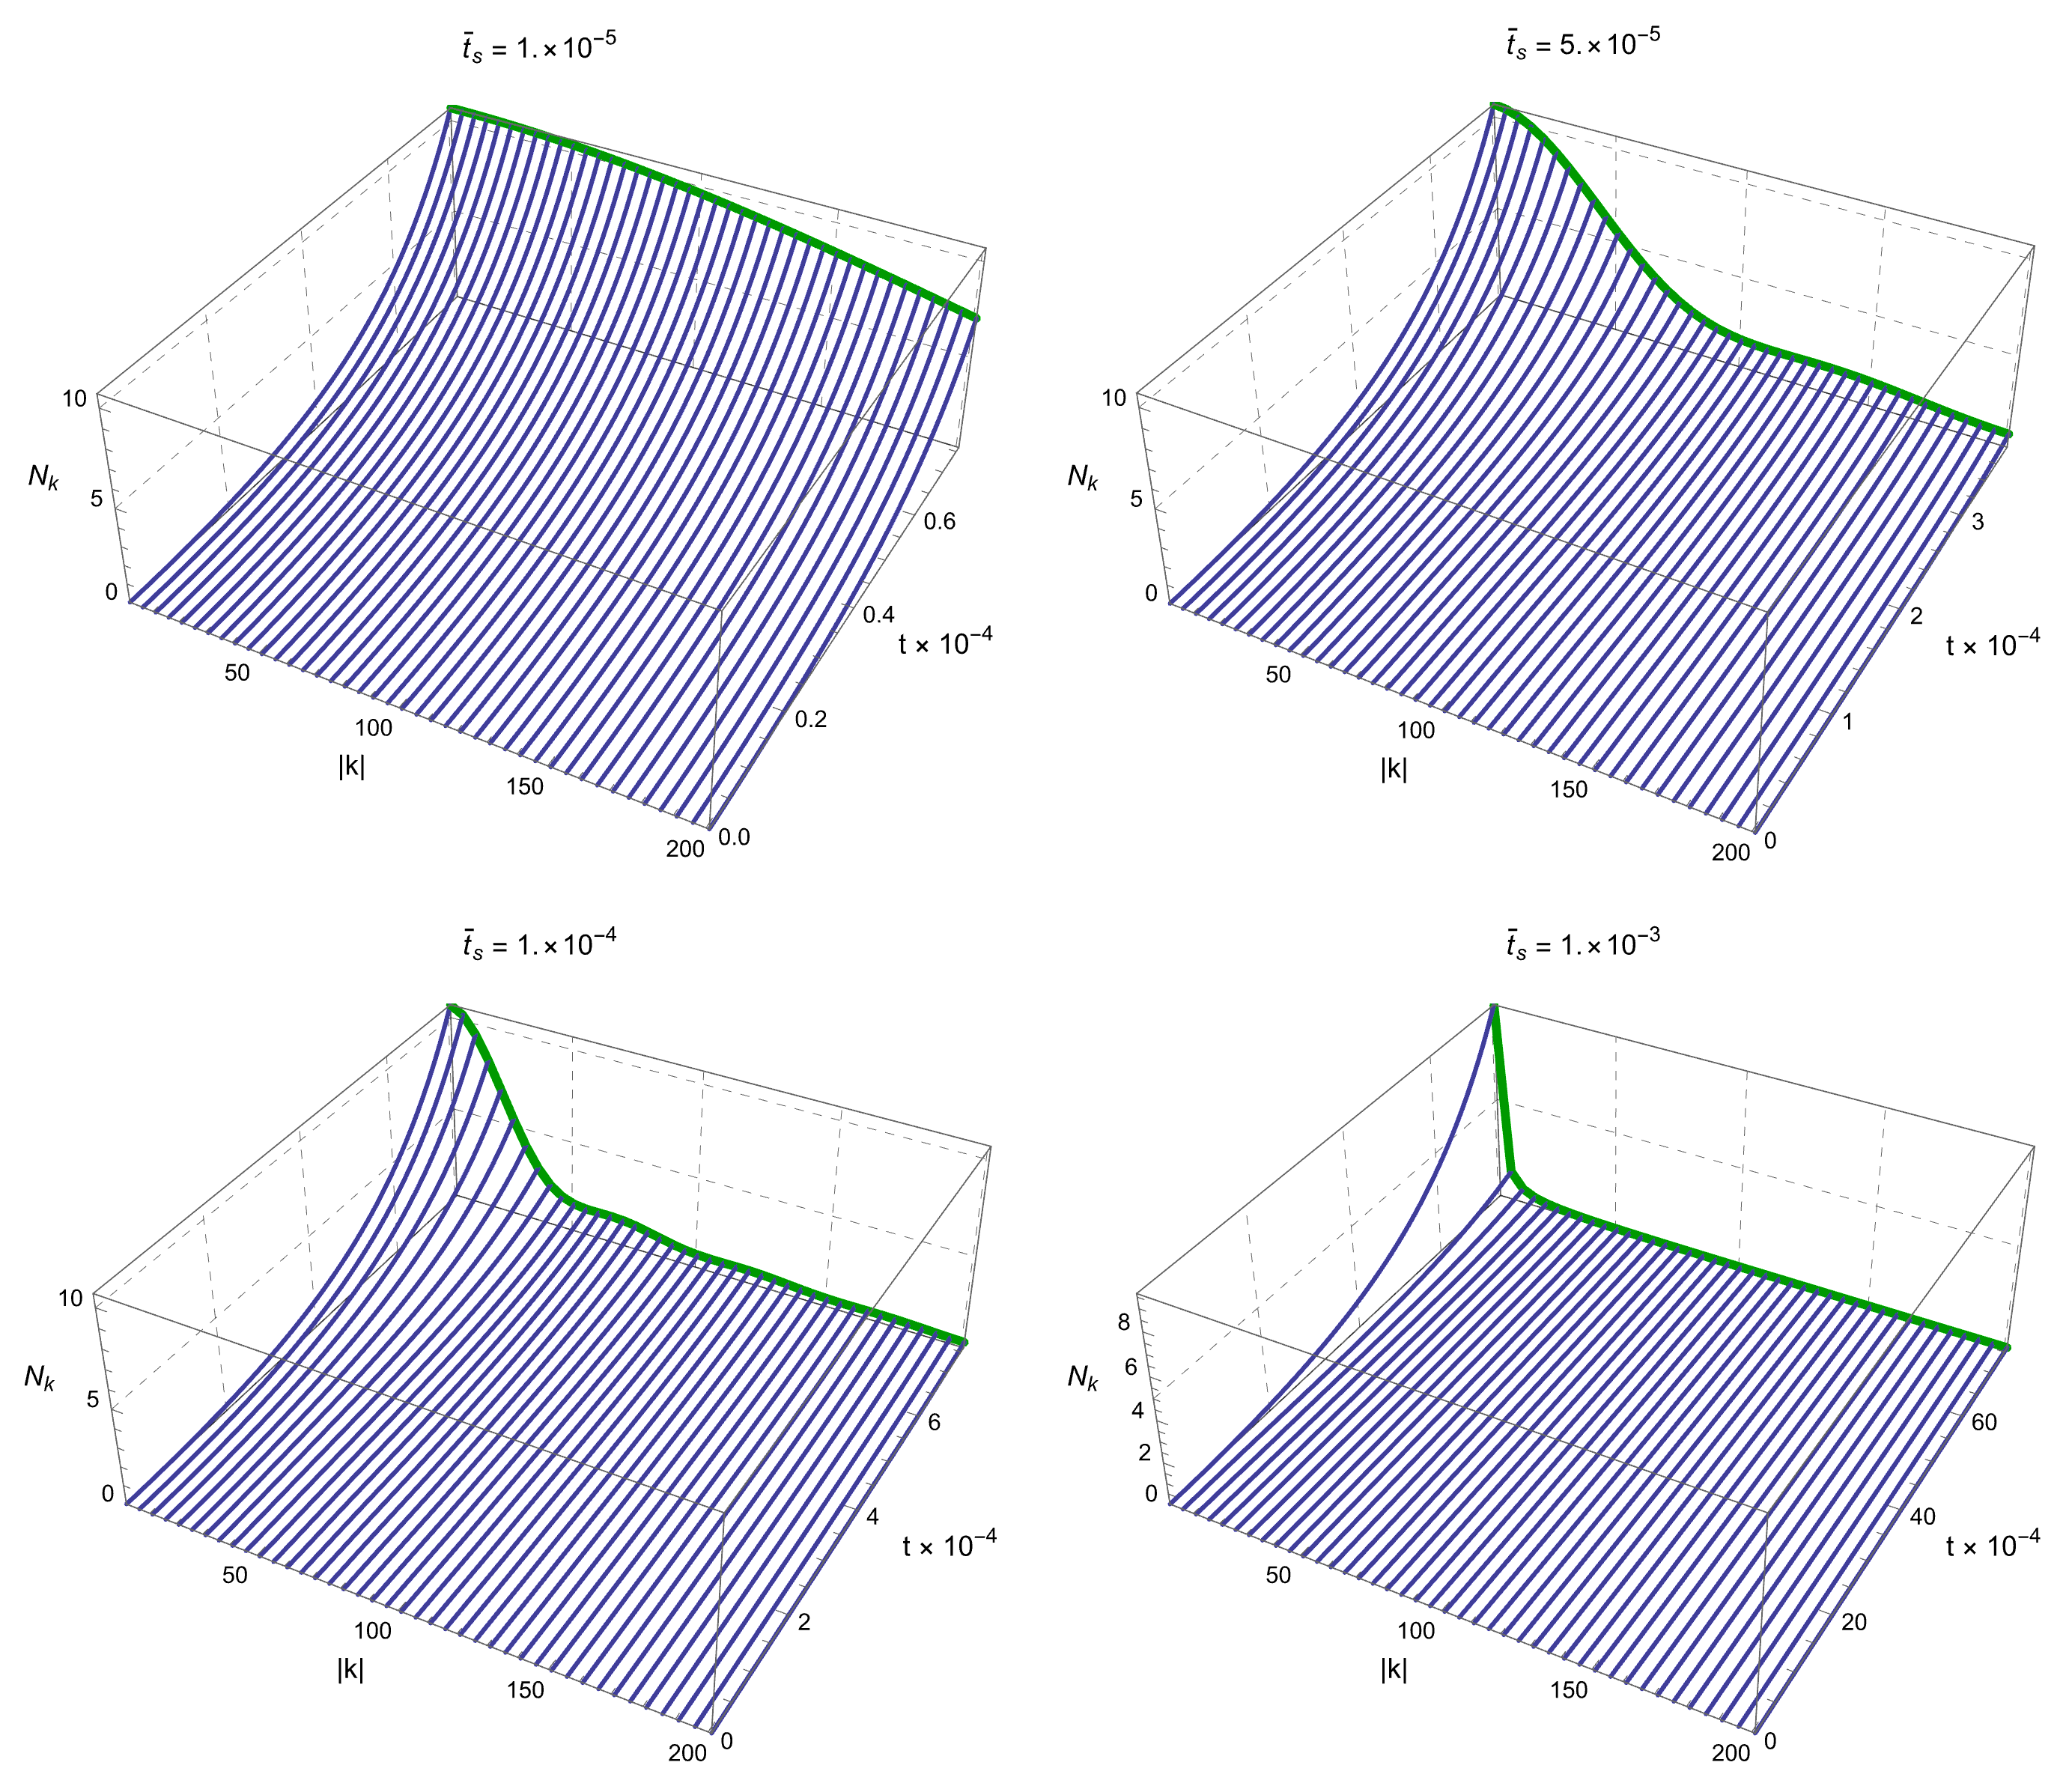
\includegraphics[width=0.5\textwidth]{Analytic_Fig_4.png}
            \caption{Momentum distribution throughout the expansion}
            \label{fig:allTime}
        \end{figure}
    \end{frame}

    \begin{frame}{Anticipated Results - Efficiency}
        \begin{itemize}
            \item Used analytic solution for particle production
            \item Calculations still took a few seconds
            \item I expect the worth to be dependant on the domains of the parameters e.g. large spatial grid over a long time needs HPC but otherwise modern technology will yield resonable calculation times
        \end{itemize}
    \end{frame}

\section{Dissemination}

    \begin{frame}{Dissemination}
        \begin{itemize}
            \item Journal-ready thesis submitted to Physical Review D
            \item Present at SOURCE
            \item Present at APS Northwest
            \item Possibly present at APS April Meeting
        \end{itemize}
    \end{frame}

\section{End Matter}
    
    \begin{frame}{Thank you \& Code source}
    \begin{columns}[onlytextwidth]
        \begin{column}{.5\textwidth}
            Thank you for your attention.
            \vspace*{0.1\textheight} \\
            The code for this project is available at:
            \begin{itemize}
                \item GitHub (QR code): \url{github.com/nondairyneutrino/thesis}
                \item My website: \url{nathanwchapman.com}
            \end{itemize}
        \end{column}
        \begin{column}{.5\textwidth}
            \centering
            \qrcode[height=0.67\textheight]{https://github.com/nondairyneutrino/thesis}
        \end{column}
    \end{columns}
    \end{frame}
    
    \begin{frame}[allowframebreaks,t]{\bibname}
        % the 'I' is caused by 'allowframebreaks'
        \AtNextBibliography{\footnotesize}% or in the preamble \AtBeginBibliography{\small}
            \nocite{*}
        \printbibliography
    \end{frame}
\end{document}

